\section{XSnare Design} \label{xsnare_design}

 \begin{figure*}[h]
	\begin{subfigure}[b]{1.0\textwidth}
		\centering
		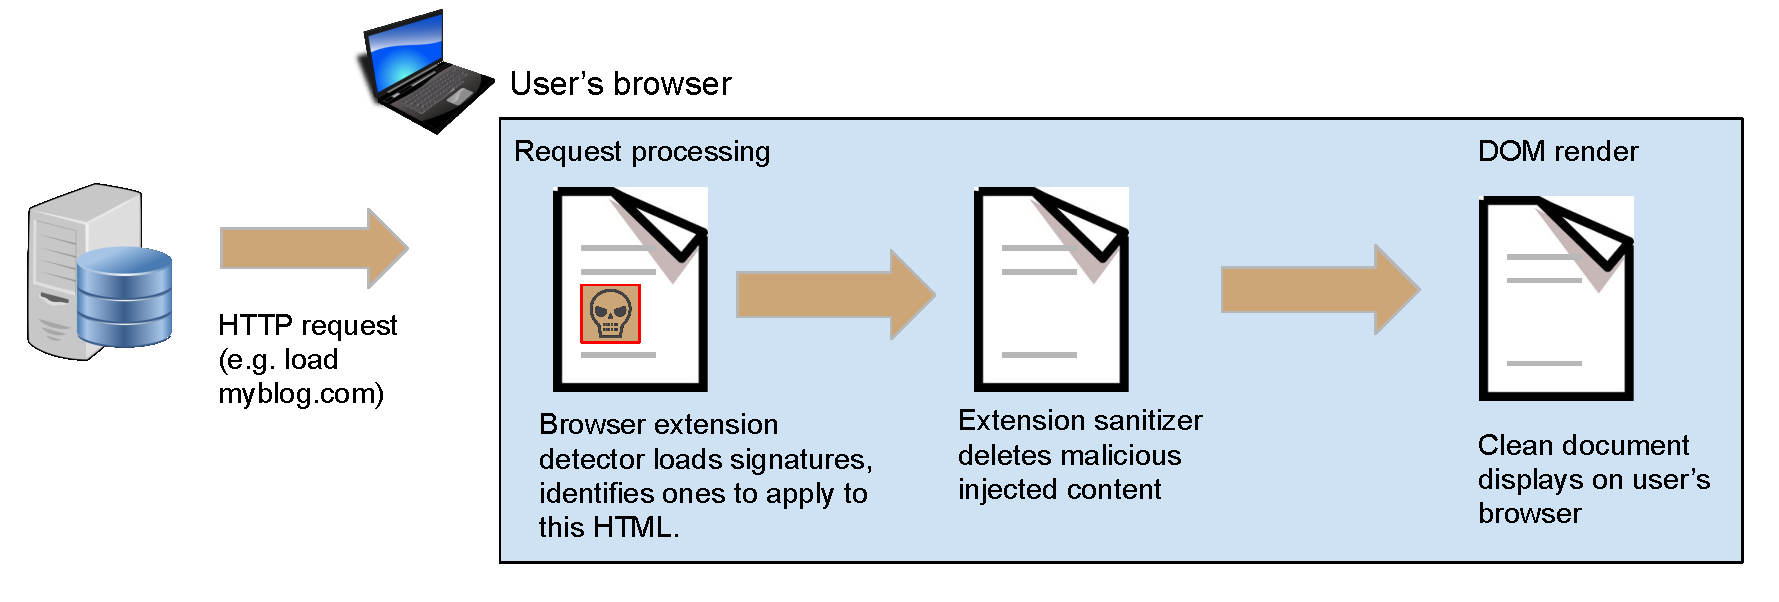
\includegraphics[scale=0.55]{img/xsnare_top.pdf}
		
	\end{subfigure}
	\hfill
	\begin{subfigure}[b]{0.3\textwidth}
		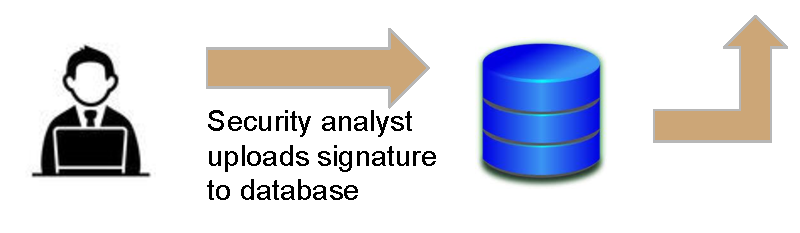
\includegraphics[scale=0.55]{img/xsnare_bot.pdf}
		
	\end{subfigure}
	\caption{\sys's approach for protection against XSS.}
	\label{fig:xsnare}
\end{figure*}

We now present \sys's components and how they interact with each other.

\subsection{Operation, at a glance} \label{operation}
  Figure~\ref{fig:xsnare} illustrates how the firewall can be used to guarantee full client-side protection: A user loads a request, such as \url{www.myblog.com}, this request might come back with malicious code in the form of an XSS attack. Before rendering the webpage in the browser, an extension can analyze the potentially malicious document. First, it loads signatures which a security analyst (a bug bounty hunter, for example) has uploaded to a database. The extension's detector analyzes the given HTML string and identifies the signatures which apply to this document. The signatures specify the injection spots in the document, and the extension's sanitizer gets rid of any malicious content. Finally, the extension passes a clean HTML document for the browser to render. Algorithm \ref{filter_algorithm} describes the network filtering process. Section \ref{implementation} explains this algorithm in more detail.
 



\iffalse
 \begin{figure*}[h]
 	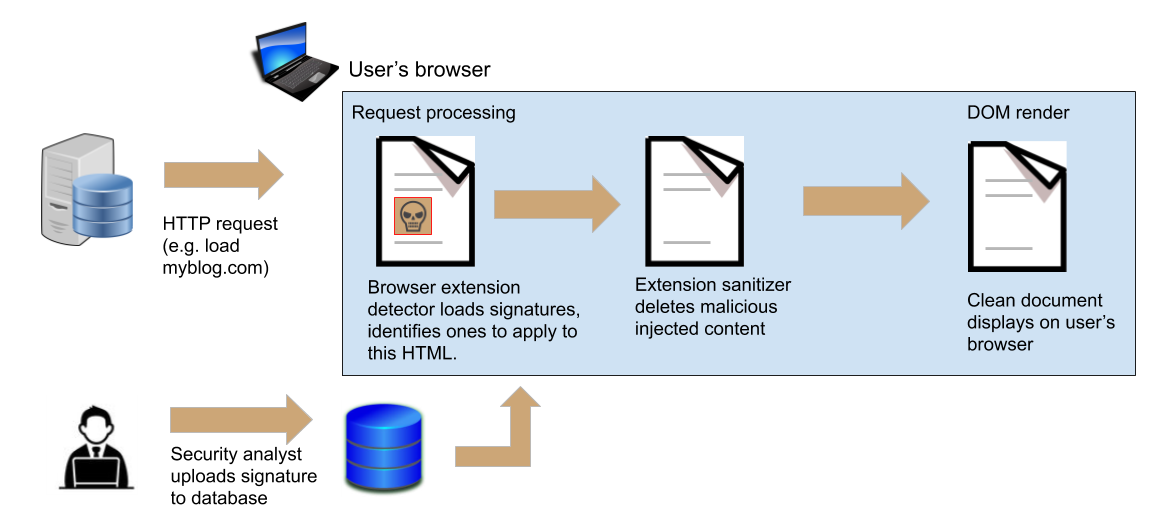
\includegraphics[scale=0.55]{img/xsnare.png}
 	\caption{\sys's approach for protection against XSS.}
 	\label{fig:dom_firewall}
 \end{figure*}
\fi

\subsection{An example application of \sys} \label{motivating_example}

In order to further explain this approach, we present a small example of how DOM context can be used to defend against XSS, taken from CVE 2018-10309 \cite{examplecve}. This is reproducible in an off the shelf WordPress installation running the Responsive Cookie Consent plugin, v1.7. This is also an example exploit which Chrome's XSS auditor does not protect against. Consider a website running PHP on the backend that takes user input and stores it to later display it to another user; in this case, the \textbf{input} element's value attribute is set by the webpage admin using the plugin's UI.

The PHP code defines the static HTML template (in black) in the "admin-page.php" file, as well as the dynamic input (in red):

\begin{lstlisting}
<input id="rcc_settings[border-size]" 
name="rcc-settings[border-size]" 
type="text" value=<@\textcolor{red}{"<?php rcc\_value('border-size'); ?>"}@>/>
<label class="description"
for="rcc_settings[border-size]">
\end{lstlisting}
\
\\
This HTML will be displayed in the admin's UI. Under normal circumstances, the \textbf{input} element might be used to insert a value of "0" as the dynamic content:
\\
\begin{lstlisting}
<input id="rcc_settings[border-size]" 
 name="rcc-settings[border-size]" 
 type="text" value=<@\textcolor{red}{"0"}@>>
<label class="description"
 for="rcc_settings[border-size]">
\end{lstlisting}
However, the php code is vulnerable to an injection attack, as it is not sanitized on the server side. If we have
\begin{lstlisting}
border-size = ""><script>alert('XSS')</script>
\end{lstlisting}
then, the browser will render the following, executing the injected script:
\begin{lstlisting}
<input id="rcc_settings[border-size]" 
name="rcc-settings[border-size]" 
type="text" value=<@\textcolor{red}{""><script>alert('XSS')</script>}@>
<label class="description"
for="rcc_settings[border-size]">
\end{lstlisting}

Note that this HTML is well-formed, so it is hard to detect that a malicious injection has occurred without knowing the application developer's intention. However, assuming an analyst has knowledge of how the full HTML should render without any injections, and the possible range of values of the injection, they can single out the point of injection, by separating user input from the server-side template, and get rid of the malicious script entirely. In the example, the injected script in red can be easily distinguished from the rest of the HTML template due to their identifiable attributes. By searching for this specific \textbf{input} element from the top of the document, and this \textbf{label} element from the bottom, the dynamic content can be identified from the static template, effectively ensnaring injection points in the HTML. 

This mechanism is partly inspired by the work in Nadji et al. \cite{Nadji:2009}. They present a client and server-side hybrid approach for XSS defence, by using server-specified policies that are enforced on the client side. Unlike other prior work, they do not rely on developers to identify untrusted sources, and tag elements server-side, such that once they reach the client, there is a clear distinction of untrusted code, which can be filtered accordingly. Our work removes the server-side component by defining the points in the HTML where untrusted code can execute.

When sanitizing the injection points, we would ideally apply functions that are equivalent to the server-side patch, but the application developer's intention might not always be clear. After careful analysis of the code in the example, we noted that while the CVE describing this vulnerability states that the bug was fixed in version 1.8 of this plugin, this was not the case: the developer fixed other similar vulnerabilities but did not handle this specific parameter. However, we can infer the application's intended behaviour from the other patches \cite{rccpatch}. In particular, the developer applied a built-in WordPress function "sanitize\_text\_field", which sanitizes the parameters by checking for common invalid characters like invalid UTF-8. The task of determining the intended behaviour falls upon a security analyst, who will act as the signature developer for a given exploit.  

In the following sections we give a detailed description of each component of our system, the challenges that arise when trying to defend against XSS client-side, and the tools provided by the browser to facilitate our methods. 
 
 \subsection{\sys Signatures} \label{signatures}
	 The signatures are at the core of our defense strategy. These must be precise enough for our system to get rid of the intended injection, without removing elements of the website crucial to the user experience. Since we are only relying on DOM knowledge, these signatures must be related to HTML features, for example, specifying elements and element attributes that are unique to where the exploit might occur. 
	 
	 The basis for our signatures relies on two observations: first, an injection has a start and end point, that is, an element can only be injected between a specific HTML node and its immediate sibling in the DOM tree; second, in a well-formed DOM, the dynamic content will not be able to rearrange its location in the document without any JavaScript execution (e.g., removing and adding elements), allowing us to isolate it from the template code. Thus, our basic approach at signature definition is to specify an injection's start and its end, and any sanitization to be done between these two endpoints. Typically, one page will have several dynamic content injection points. The signature developer has to be able to identify all of these. Different scenarios might warrant different resolutions, ranging from stopping a webpage's rendering altogether, to performing some basic checks on the string. We discuss how different exploits might affect a signature definition and how our signature language gives an analyst enough expressibility to deal with these in later sections.
	 
	 We believe CVEs to be an ideal source for signatures. Since previous client-side work does not focus on application-specific protection, these tools often use generic approaches to detecting exploits. However, once new vulnerabilities are found, these systems often lack the maintainability obtained by leveraging active CVE development. 
	 
	 Our system assumes signatures are written by a third-party: bug bounty hunters and penetration testers will commonly identify issues in application code, inform developers and publish it for the benefit of the community in the form of CVEs. Our system adds an extra component to this workflow, where hackers and security enthusiasts also write the signatures to defend users. Thus, the signature database is maintained by a trusted entity which audits CVEs, and thus, a malicious analyst can not take advantage of this model to throttle the extension's performance. An analyst can write a signature in our language given their knowledge on the exploit, as they will often know both the source and the way it manifests in the HTML, as well as the fix.
 
 \subsection{Firewall Signature Language} \label{signature_language}
 Our signature language needs to be such that it has enough power of expression for the signature writer to be precise, both for determining the correct web application and to identify the affected areas in the HTML. Due to the nature of our signature definitions, a language based on regular expressions (a regex language) suffices to express precise sections of the HTML. Furthermore, a regex language allows us to identify malformed HTML before it renders on the browser. The following is the signature that defends against the motivating example of Section 2.2:
 \lstset{basicstyle=\small}
\begin{lstlisting}[breaklines=true,caption={An \sys signature},label={lst:xsnare_signature}]
url: 'wp-admin/options-general.php?page=rcc-settings',
software: 'WordPress',
softwareDetails: 'responsive-cookie-consent',
version: '1.5',
type: 'string',
typeDet: 'single',
sanitizer: 'regex',
config: '/^[0-9](\.[0-9]+)?$/',
endPoints: 
['<input id="rcc_settings[border-size]" name="rcc_settings[border-size]" type="text"
  value="',
'<label class="description" 
for="rcc_settings[border-size]">']
\end{lstlisting}

A detailed description of the process by which this signature's attributes were defined is given in Section \ref{case_study}. In summary, a signature will have the necessary information to determine whether a loaded page has a vulnerability, and the HTML identifiers to properly sanitize an injection point and eliminate potentially malicious content. Note that it is possible for one document to have multiple injection points, which complicates the detection mechanism: for example, if one document has two different injection points, a knowledgeable attacker might leverage this information to try to trick the extension into identifying the wrong spots. We further discuss measures to protect against these attacks in the implementation section.
  
Once the page's identifying information and the dynamic content is established by an analyst, they can configure their signatures with a function chosen from a pre-defined static set of sanitization functions. These functions innoculate potentially malicious injections based on the DOM context surrounding the injection. The goal of signatures is to provide such sanitization, while maintaining the core web page user experience. To this end, default injection point sanitization is done with DOMPurify \cite{10.1007/978-3-319-66399-9_7} \footnote{This library is described by its creators as a "DOM-only, super-fast, uber-tolerant XSS sanitizer for HTML, MathML and SVG". The Mozilla community cites it as an useful tool for "safely inserting external content into a page" \cite{safecontent}}. While it offers a lot of configurability and hooks, we have used the default functionality, with satisfying results, as described in Section 4, in our own signatures. However, there are cases where page functionality is lost due to a naive sanitization approach. Thus, it is sometimes more desirable to use a different sanitization approach, especially when heavier methods disrupt the look and feel of the web page.
 
  We provide different types of sanitization: "DOMPurify", "escape", and "regex". Regex Pattern matching can be particularly effective when the expected value has a simple representation, e.g. a name field should only have a particular subset of characters available. Additionally, for each of these approaches, the signature can specify a corresponding config value, as described in Section 5.1. DOMPurify provides a rich API for additional configuration. When escaping, defining specific characters to escape via regex can be useful. For pattern matching via regex, the config value specifies the string the injection point content should match.
 
 An alternative to this approach would have been to allow signatures to specify arbitrary code for the sanitization routines. While this would provide a more accurate sanitization technique, we have decided to impose a declarative spec for these routines for three main reasons:
\begin{enumerate} 
	\item Security Concerns: We assume signatures come from a trusted source. However, partly due to the way they are currently stored, it is possible for an attacker to add malicious signatures. In general, this would only cause pages to trigger signatures that should not have been triggered, potentially harming the web site user experience. If we allowed arbitrary code to run from signatures, an attacker could take control of the victim's browser, as the code would execute in a high-privilege environment.
	\item Case Coverage: While our provided methods might be limited in some scenarios, we have applied them in our studied CVEs with positive results, and are confident they can cover most use cases.
	\item Adoption: A declarative language will help signature developers expedite the process of writing signatures, as they will find that our provided methods will most often suffice.
\end{enumerate}
 
 \subsection{Firefox Extension} \label{firefox_extension}
 Our system's main component is a browser extension which rewrites potentially infected HTML into a clean document. We believe an extension to be ideal for the purpose of defending against attacks due to the context available to it. Previous client-side work has focused on browser modifications and higher-level tools. Without access to the page's context, an XSS protection tool does not have the information required for the application-specific behaviour we seek. The extension's main purpose is to detect exploits in the HTML by using signature definitions and maintain a local database of signatures that is periodically updated from the main server. The extension translates signature definitions into patches that rewrite incoming HTML on a per-URL basis, according to the top-down, bottom-up scan described earlier. 

The patch applied by the extension needs to take place in the raw HTML string. Even before any code runs, the parsing of the HTML into a DOM tree might cause elements to be re-arranged into an unexpected order, making our extension sanitize the wrong spot. For example, a <tr> element may only have direct children <th> or <td>. In our experiments, we found that an injection occurring as a direct child of the <tr> might cause the injected element to be rendered before the <tr> in the DOM. The following code shows the HTML as written in its file, with the injection (the \textbf{img} element) in red:

\begin{lstlisting}
<table class="wp-list-table">
  <thead>
     <tr>
     <th></th>
     <@\textcolor{red}{<img src="1" onerror="alert(1)">}@>
     <th>
   	    <form method="GET" action="">
...
\end{lstlisting}

According to this HTML, the signature developer might identify the exploit as occurring inside the table with the specified class, and the extension would be able to sanitize the code correctly. However, if we wait until the string has been parsed into a DOM tree, the elements are rearranged due to the previously mentioned rule:

\begin{lstlisting}
<@\textcolor{red}{<img src="1" onerror="alert(1)">}@>
<table class="wp-list-table">
   <thead>
   <tr>
   <th></th>
   <th>
      <form method="GET" action="">
...
\end{lstlisting}

Note that the injected img element is now outside of the table, simply by virtue of the DOM parsing. When performing the top-down search, the extension will search past the injection, as it occurs before the table element, and will therefore miss it during sanitization, creating a false negative. Similarly, false positives might occur if elements which were outside of an injection point are rearranged inside one. Thus, we can't wait until the website is rendered client-side to start interposing on code execution, and therefore, our detector acts as an in-browser network filter.

A knowledgeable attacker can not take advantage of such behaviour: even if they know what the signatures look like, the extension can't be tricked into looking for the element in the wrong spot, as the injection can only happen after a signature's start and before its end. Additionally, the injection must end at a certain point in the document. Since we look for the end point from the bottom-up, we will eventually reach the injection's end, and, regardless of the contents (for example, trying to spoof the end point early), the sanitization will be correctly applied.

\subsection{Handling multiple injections in one page} \label{multiple_injections}
In Listing \ref{lst:xsnare_signature}, the endPoints were listed as two strings in the incoming network response. However, there are cases where arbitrarily many injection points can be generated by the php code, such as a for loop generating table rows. For these, it is hard to correctly isolate each endPoint pair, as an attacker could easily inject fake endPoints in between the original ones.

\begin{figure}[h]
	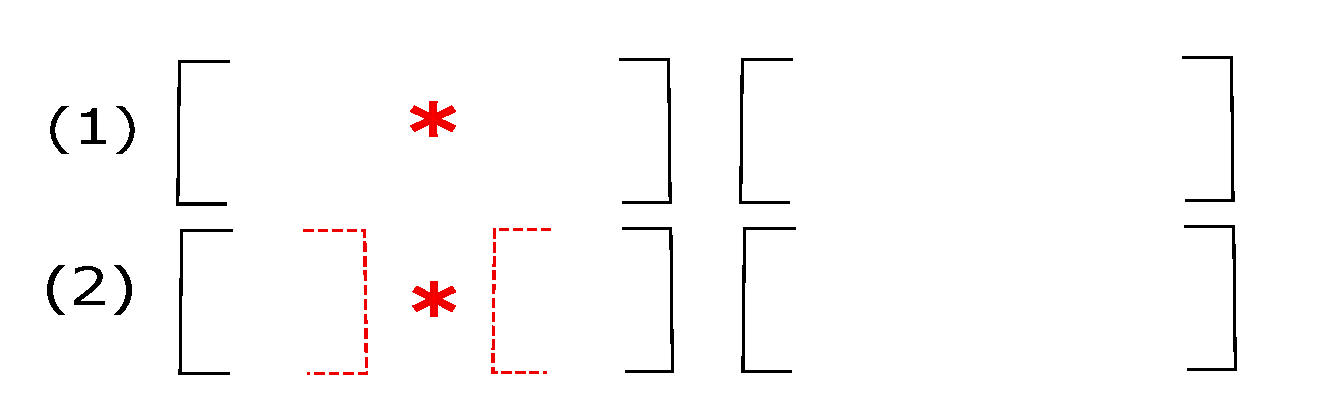
\includegraphics[scale=0.25]{img/attacker_injection_compound.pdf}
	\caption{Example attacker injection when multiple injection points exist in the page. (1) shows a basic injection pattern. (2) shows an attempt to fool the detector.}
	\label{fig:attacker_injection}
\end{figure}



We illustrate one case of this mechanism using Figure~\ref{fig:attacker_injection} as a visual aid: In (1), the content in black is a template. The content in between the brackets is an injection point, where dynamic content is injected into the template. In the case of a vulnerability, the injected content (the star) can expand to any arbitrary string. The signature separates the injection from the rest by matching for the start and end points (called the endPoints), represented by the brackets. This HTML originally has two pairs of endPoint patterns.

In (2), the attacker knows these are being used as injection endPoints and decides to inject a fake ending point and a fake starting point, with some additional malicious content in between (shown in red). If the detector were to look for several pairs of endPoints, it would not be able to tell the difference between the red and black patterns, even when using our top-down, bottom-up approach, and would not be able to get rid of the content injected in the star. Therefore, we have to use first starting point and the last ending point and sanitize everything in between. Depending on the application, this might get rid of a substantial amount of valid HTML, in particular, the web page's functionality might be affected. Note that due to the difficulty of applying a general solution to this scenario, we defer to the signature developer's judgement, of what behaviour the detector should follow. We expand upon this further in Section 5.


\begin{figure}[h]
	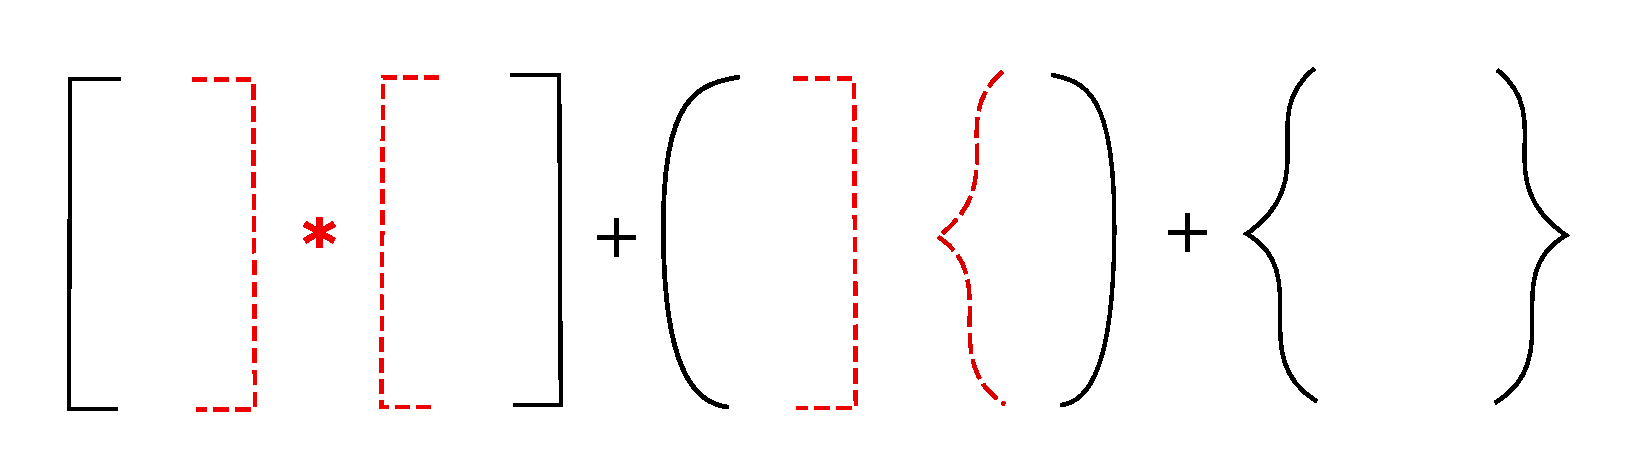
\includegraphics[scale=0.25]{img/attacker_injection_unique.pdf}
	\caption{Example attacker injection when multiple distinct injection points exist in the page}
	\label{fig:attacker_injection_unique}
\end{figure}


Figure ~\ref{fig:attacker_injection_unique} illustrates a case when there are several injection points in one page, but each of them is distinct. Now, because the filter is only looking for one pair of brackets, the attacker can't fool the extension into leaving part of the injection unsanitized. However, they could inject an extra ending bracket after the opening parenthesis, or similarly, an extra opening brace before the ending parenthesis. In either case, the extension will be tricked into sanitizing non-malicious content, the black pluses (+). We can detect this behaviour by noting that we know the order in which the endPoints should appear, and so if the filter sees a closing endPoint before the next expected starting endPoint, or similarly, a starting endPoint before the next expected closing endPoint, this attack can be identified. In the diagram, the order is brackets, parenthesis, braces. When it sees a closing bracket after an opening parenthesis, and similarly, when it sees an opening brace before a closing parenthesis, this represents the described attack. As with the previous scenario, we can not easily identify which endPoint is the real one, so sanitization will still potentially get rid of non-malicious content. As before, the signature developer specifies whether the page should be blocked or sanitization goes through as usual when this behaviour is detected.

\subsection{Dynamic injections} \label{dynamic_injections}

The top-level documents of web pages fetch additional dynamic content
via \js{fetch} or AJAX APIs. Content fetched in
this way is also vulnerable to \xss, and must be filtered. An example
vulnerability is CVE-2018-7747 (Wordpress Caldera Forms, which allows malicious
content retrieved from the plugin's database to be injected in response to a click.

\sys allows XHR requests to be filtered with \js{xhr}-type
signatures. To reduce the number of signatures that need to be
considered when a browser issues a request, we require that signatures
for XHR be nested inside a signature for a top-level document. If a
page's main content matches an existing top-level signature description,
\sys will then enable all nested XHR listeners.

Signatures for dynamic requests are specified in the \js{listenerData}
key, which includes a listener type and method. The idea is extensible
to scripts and other objects loaded separately from the main document
(e.g., images, stylesheets, etc.).

\lstset{basicstyle=\small}
\begin{lstlisting}[breaklines=true,caption={
      An example dynamic request signature. This patches CVE-2018-7747.
    },label={lst:dynamic_signature}]
...
listenerData: [{
  listenerType: 'xhr', listenerMethod: 'POST',
  sanitizer: 'escape', type: 'string',
  listenerUrl: 'wp-admin/admin-ajax.php',
  typeDet: 'single-unique',
  endPoints: ['<p><strong>', '[AltBody]']
}]
\end{lstlisting}

